\documentclass[12pt]{article}
\usepackage{graphicx}
\usepackage{color}

\begin{document}
\begin{titlepage}
\begin{center}
\begin{huge}
\begin{center}
\textcolor{blue}{V3D Digraph Visualizer Architecture and Design}
\end{center}
\end{huge}
\hfill \break
\begin{Large}
\begin{center}
\textcolor{blue}{Team: App-Synth}
\end{center}
\end{Large}
\begin{small}
\begin{flushleft}
Author(s):
\end{flushleft}

\begin{itemize}
	\item Kulani Bamuza \\
	\item Keanan Jones \\
	\item Munyaradzi Mpofu\\
	\item Neo Thokoa\\	
	\item Takalani Sigama\\
	
\end{itemize}
\end{small}

\end{center}
\begin{center}
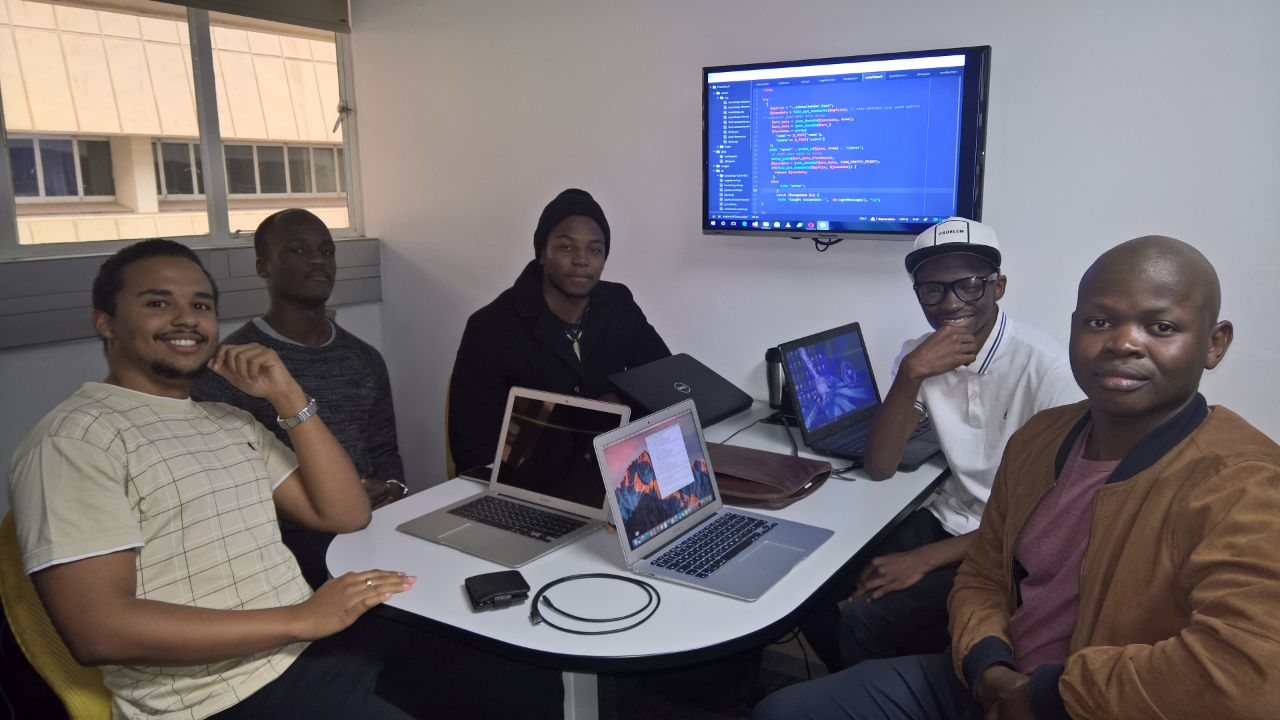
\includegraphics[scale=0.4]{Dps/TeamPic.jpg}
\\
\textcolor{blue}{\textit{University of Pretoria, Department of Computer Science
\\
15 May 2017}}

\end{center}
\end{titlepage}

\newpage
\pagenumbering{arabic}
\thispagestyle{empty}
\tableofcontents
\clearpage

\textcolor{blue}{\section{Architecture}}
\begin{flushleft}
For the V3D Digraph Visualiser, the Master-slave architecture is employed. This is due to the downstream flow of information from the "master" node(V3D app on phone) to the external display ("slave" node). \newline
All control is on the V3D mobile app, therefore this will be the master node of the system. The mobile application will stream instructions to the desktop application. 
We do this to achieve near real time synchronization between the two displays. The slave, ie. the desktop application, will receive the instructions, decode them and update the view accordingly.
\end{flushleft}

\includegraphics[width=150mm,scale=0.5]{"Deployment Diagrams/Deployment Diagram".png}

\newpage

\textcolor{blue}{\section{Quality Requirements}}
\begin{flushleft}
The V3D Digraph Visualiser has a number of quality requirements which will have a major impact on the overall impression of the system. These include:
\begin{itemize}
	\item Extensibility
	\item Reliability
	\item Usability
\end{itemize}
\end{flushleft}

\textcolor{blue}{\section{Creation Module}}
\subsection{Scope}
The purpose of this module is to handle the creation of new graphs in the virtual environment. This module is responsible for the creation of graph nodes and the creation of edges between these nodes. The module is also responsible for the removal of nodes from the graph and saving the created graph to a graph specification file in order for the graph to be visualised again at a later stage.
\subsection{Domain Models}

\includegraphics[width=150mm,scale=0.5]{"Deployment Diagrams/CreationModule".png}

\textcolor{blue}{\section{Control Module}}
\subsection{Scope}
The purpose of this module is to handle all of the controls within the system. These include menu controls, graph controls and node controls. Menu controls are used to navigate between different scenes in the virtual environment, graph controls which are used to rotate and reposition the graph and node controls are used to interact with graph nodes by performing actions such as picking up, dropping and repositioning nodes. 
\subsection{Domain Models}

\includegraphics[width=150mm,scale=0.5]{"Deployment Diagrams/ControlModule".png}

\textcolor{blue}{\section{Renderer Module}}
\subsection{Scope}
The renderer module is responsible for creating the digraph model in the virtual environment. This module renders all of the nodes and relationships between all the nodes and clusters nodes of a particular type. In addition, this module will also display the attributes of a selected node and display the name of each node directly above the node. 
\subsection{Domain Models}

\includegraphics[width=150mm,scale=0.5]{"Deployment Diagrams/RendererModule".png}

\textcolor{blue}{\section{Serialization Module}}
\subsection{Scope}
The serialization module is responsible for the serialization of JSON data into objects. These JSON objects will contain the necessary information for the graph model to be created in the virtual environment. This module will also be responsible for serializing the objects to JSON format for the purposes of creating a graph specification file. 
\subsection{Domain Models}

\includegraphics[width=150mm,scale=0.5]{"Deployment Diagrams/SerializationModule".png}

\section{Technologies}
For the purposes of the development of this application, the Unity Game Engine is used. Unity is used to create and render all of the graphical components of the system. A 3rd party 3D modelling software called Blender is also used for the creation of the graphical components which are rendered within the application. The Newtonsoft C-Sharp library is used for the purpose of serializing and de-serializing of the graph specification files which are stored in JSON format. The TeamViewer mobile and desktop applications were used to display the mobile screen on an external display, where the mobile device took on the role of a server sending screen data and the desktop application took on the role of a client receiving screen data.
\end{document}